\chapter{Initialisation et relation clients/serveur}
 
\section{Client}
Le client est la partie propre à chaque équipe qui permet de jouer, aussi bien seul que contre un client extérieur. Ce dernier créé son propre plateau au début du jeu et communique avec son adversaire à chaque coup afin de tenir son plateau à jour. Il lui faut donc une phase de démarrage puis une phase de jeu en attendant un signe du serveur lui annonçant sa potentielle victoire.
\subsection{Initialisation}
Dans cette phase de démarrage, le client va procéder à l'initialisation de beaucoup de paramètres afin de pouvoir par la suite suivre le déroulement de la partie.\\
Pour cela, le serveur va envoyer les informations de jeu telles que :
\begin{itemize}
    \item \texttt{Id} : Correspondant au numéro de joueur (ici 0 ou 1).
    \item \texttt{Num queens} : Le nombre de reines attribuées à chaque joueur.
    \item  \texttt{Queens} : Cette fois-ci c'est un tableau de tableau afin de stocker la position des reines des deux joueurs.
    \item  \texttt{Size} : Correspondant à la longueur d'un côté du plateau.
    \item  \texttt{Graph} : Le graphe de liaisons généré en fonction du plateau.
\end{itemize}

\bigbreak

Le client stocke ces informations et les utilise pour créer \texttt{world}, le tableau représentant la partie. Ce tableau recense la position des flèches et des reines sans faire de différence étant donné sa représentation. Il est fait de telle sorte que chaque position du tableau est associée à une case du plateau. Ainsi, le client a juste à regarder dans le tableau à l'endroit de la case qu'il souhaite accéder pour savoir si cette dernière est disponible. 

\subsection{Stratégies}

Le client procède ensuite au jeu. Pour cela, il doit savoir le coup de son adversaire pour actualiser son plateau si ce n'est pas à lui de jouer le premier coup. Une fois l'actualisation faite vient la phase de mouvement.\\
Ici deux stratégies ont été implémentées afin de voir le comportement d'une partie avec deux clients différents. 
\begin{itemize}
    \item \texttt{Simpliste} : Première stratégie implémentée dans le but d'avoir un déplacement assez tôt dans la production du projet, donc pas très complexe. Ce déplacement se fait donc par la première reine disponible, d'une seule case et dans la première direction disponible d'après le graphe de liaisons ainsi que le tableau \texttt{world}.
    \medbreak
    \item \texttt{Random} : Cette dernière a été implémentée dans le but de complexifier les parties. Elle va cette fois-ci choisir une reine aléatoirement, qu'elle va déplacer dans une direction disponible aléatoire, et d'un nombre de cases également aléatoire tant qu'elle ne rencontre pas une autre reine ou un obstacle. Un exemple de déplacement est montré \textbf{Figure\ref{fig:gamestrat}}. 
    \medbreak
\end{itemize}
Après avoir bougé, la reine en question va pouvoir tirer. De la même façon que pour les déplacements, il y a deux méthodes de tir, chacune similaire au déplacement qui lui est associé. Cependant, pour la méthode \texttt{random}, la flèche tirée dans une direction aléatoire et sur une distance aléatoire, s'arrêtera si elle est à côté d'une reine ennemie. Cela a été fait dans le but de gagner plus rapidement la partie.

\begin{figure}[H]
    \centering
    \begin{subfigure}{0.4\textwidth}
        \centering
        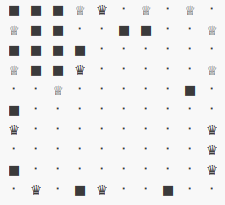
\includegraphics[scale=0.5]{Plato1.png}
        \caption{État d'un plateau $10 \times 10$ après 18 coups. }
        \label{subfig:toblo}
    \end{subfigure}
    \hspace{1cm}
    \begin{subfigure}{0.52\textwidth}
        \centering
        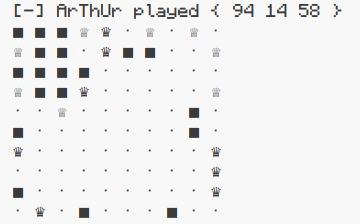
\includegraphics[scale=0.5]{Nouvelle_photoduplato.png}
        \caption{19ème coup de la partie joué en aléatoire.}
        \label{subfig: coupdeouf}
    \end{subfigure}
    \caption{Affichage du 19ème coup (ici de la case $94 \rightarrow 14$ et tir case $58$).}
    \label{fig:gamestrat}
\end{figure}
\medbreak
Une fois toutes ces actions faites, le monde du client est modifié en conséquence pour garder le fil de la partie et l'ensemble d'actions faites par le joueur sont envoyées au serveur.


\section{Serveur}

Le serveur est conçu pour faire le lien entre les clients et actualiser la partie de jeu tour à tour. Il doit également vérifier les coups proposés par les joueurs, et signaler lorsque l'un des deux a remporté la partie.

\medbreak

Les règles définissant le jeu garantissent la terminaison d'une partie, il a donc été possible de boucler seulement sur les conditions de victoire des joueurs. À chaque tour de boucle, le joueur désigné fait une proposition de mouvement, caractérisée par une structure nommée \texttt{move}, regroupant : la position source de la reine, la destination souhaitée, et l'endroit sur lequel elle a tiré.

\medbreak

A ce moment, c'est au serveur de vérifier si le coup proposé est valide : la destination de la reine et le chemin qu'elle emprunte pour y aller se doivent d'être libre et dans le plateau, de même que pour la destination de la flèche tirée. Si c'est le cas, il actualise le plateau de jeu pour l'affichage, et c'est au tour de l'autre joueur. Si ce n'est pas le cas, la boucle de jeu s'arrête, et c'est l'adversaire qui gagne instantanément.  

%\subsection{Boucle de jeu}

%Dans la boucle de jeu, les joueurs jouent chacun leur tour, 
%\subsection{Verification}

%Lors de la partie les joueurs envoient leurs modifications de jeu dès lors que leur tour est fini. Si le client respecte les règles et que son monde est tenu à jour correctement, le jeu continue. Cependant pour prévenir d'une éventuelle tentative de triche ou simplement d'un coup qui n'est pas correcte, le serveur se doit d'avoir un processus de verification des coups.\\

\section{Compilation}

% Les graphes de dépendances vu en partie \ref{sec:gsl} nécessitent la bibliothèque \textit{GNU Scientific Library}. La compilation du serveur 

% \medbreak

Les clients ayant pour but d'être interopérables et réutilisés sur différents serveurs, ils sont compilés séparément en tant que bibliothèque partagée. Pour cela, on utilise le paramètre \texttt{-shared} de \texttt{gcc}.\\
Cela présente plusieurs avantages pour les clients, notamment une réduction de la taille du binaire de l'application et la possibilité mettre à jour le client sans avoir à recompiler l'ensemble de l'application.

\medbreak

Cependant, l'utilisation de bibliothèques partagées peut également présenter des défis en termes de compatibilité et de dépendances. Les clients doivent être conçus de manière à être compatibles avec la version de la bibliothèque partagée disponible sur le système d'exécution. Les problèmes de dépendance peuvent également se poser si une bibliothèque partagée utilisée par un client est mise à jour avec une version incompatible, ce qui peut entraîner des erreurs d'exécution.

\section{Tests}

Les tests sont indispensables car ils permettent de vérifier facilement, et à chaque nouvelle implémentation, qu'aucune fonctionalitée n'est perdu. Ceci évite donc de \textit{rétrograder} en terme de fonctionalités, et de vérifier précisemment l'intégritée du code. \\
Chaque fonction de test vise une fonction d'un fichier source en particulier, afin d'isoler de manière efficace les potentiels problèmes. Chaque comportement est vérifié avec des \texttt{assert()}, qui permettent de suspendre le programme en cas d'erreur ou de résultats discordants. 